\section{Classes}


%=||======================================================================>
\subsection{Server tier class diagram}
This diagram shows the web server tier of WHAT. It controls the web server and it can only access
 the facade of the tier below.
\begin{center}
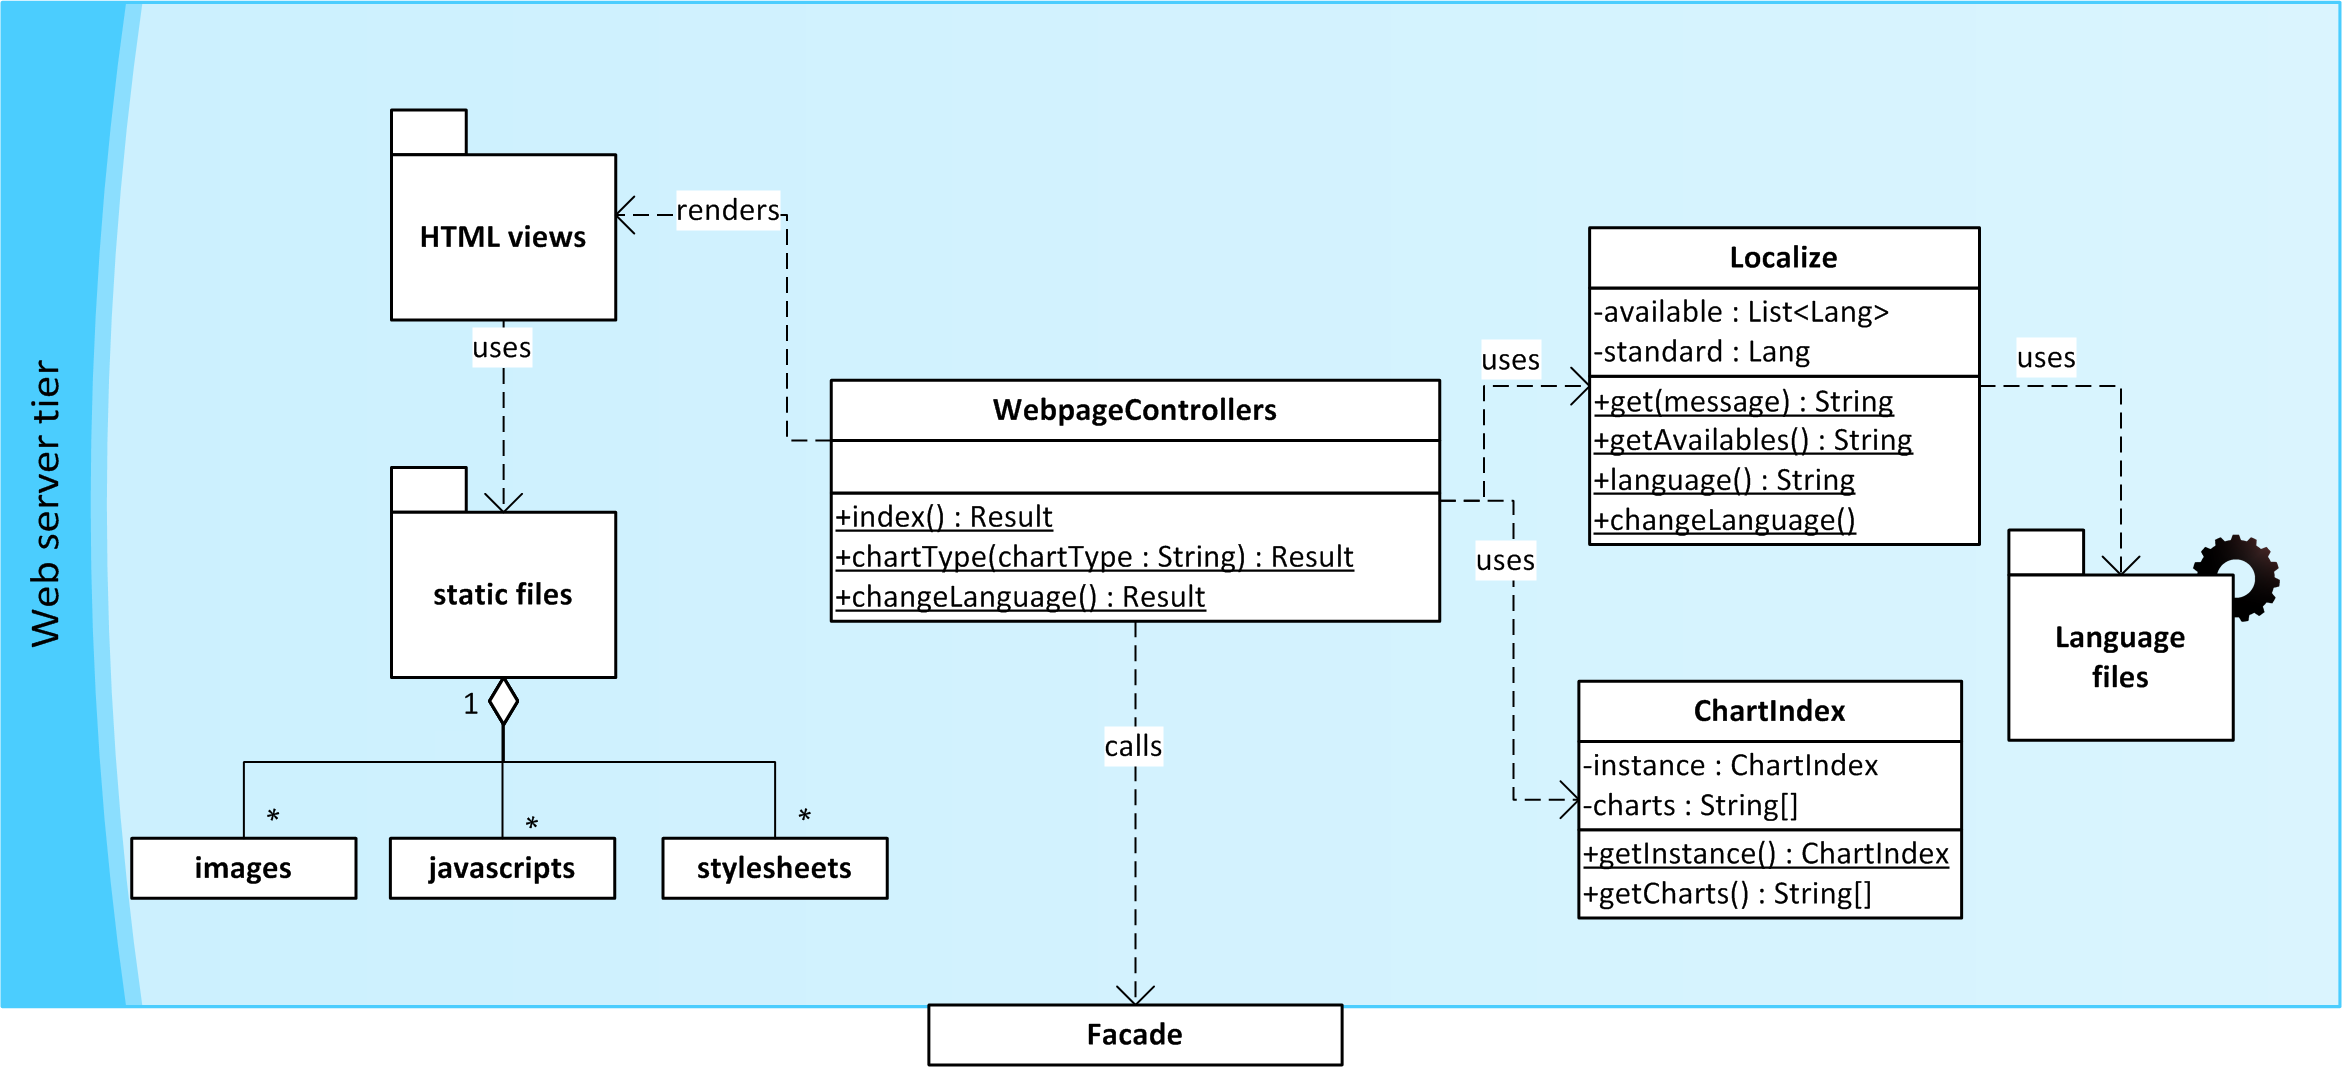
\includegraphics[width=1\linewidth]{Pictures/ServerTierDia.png}
%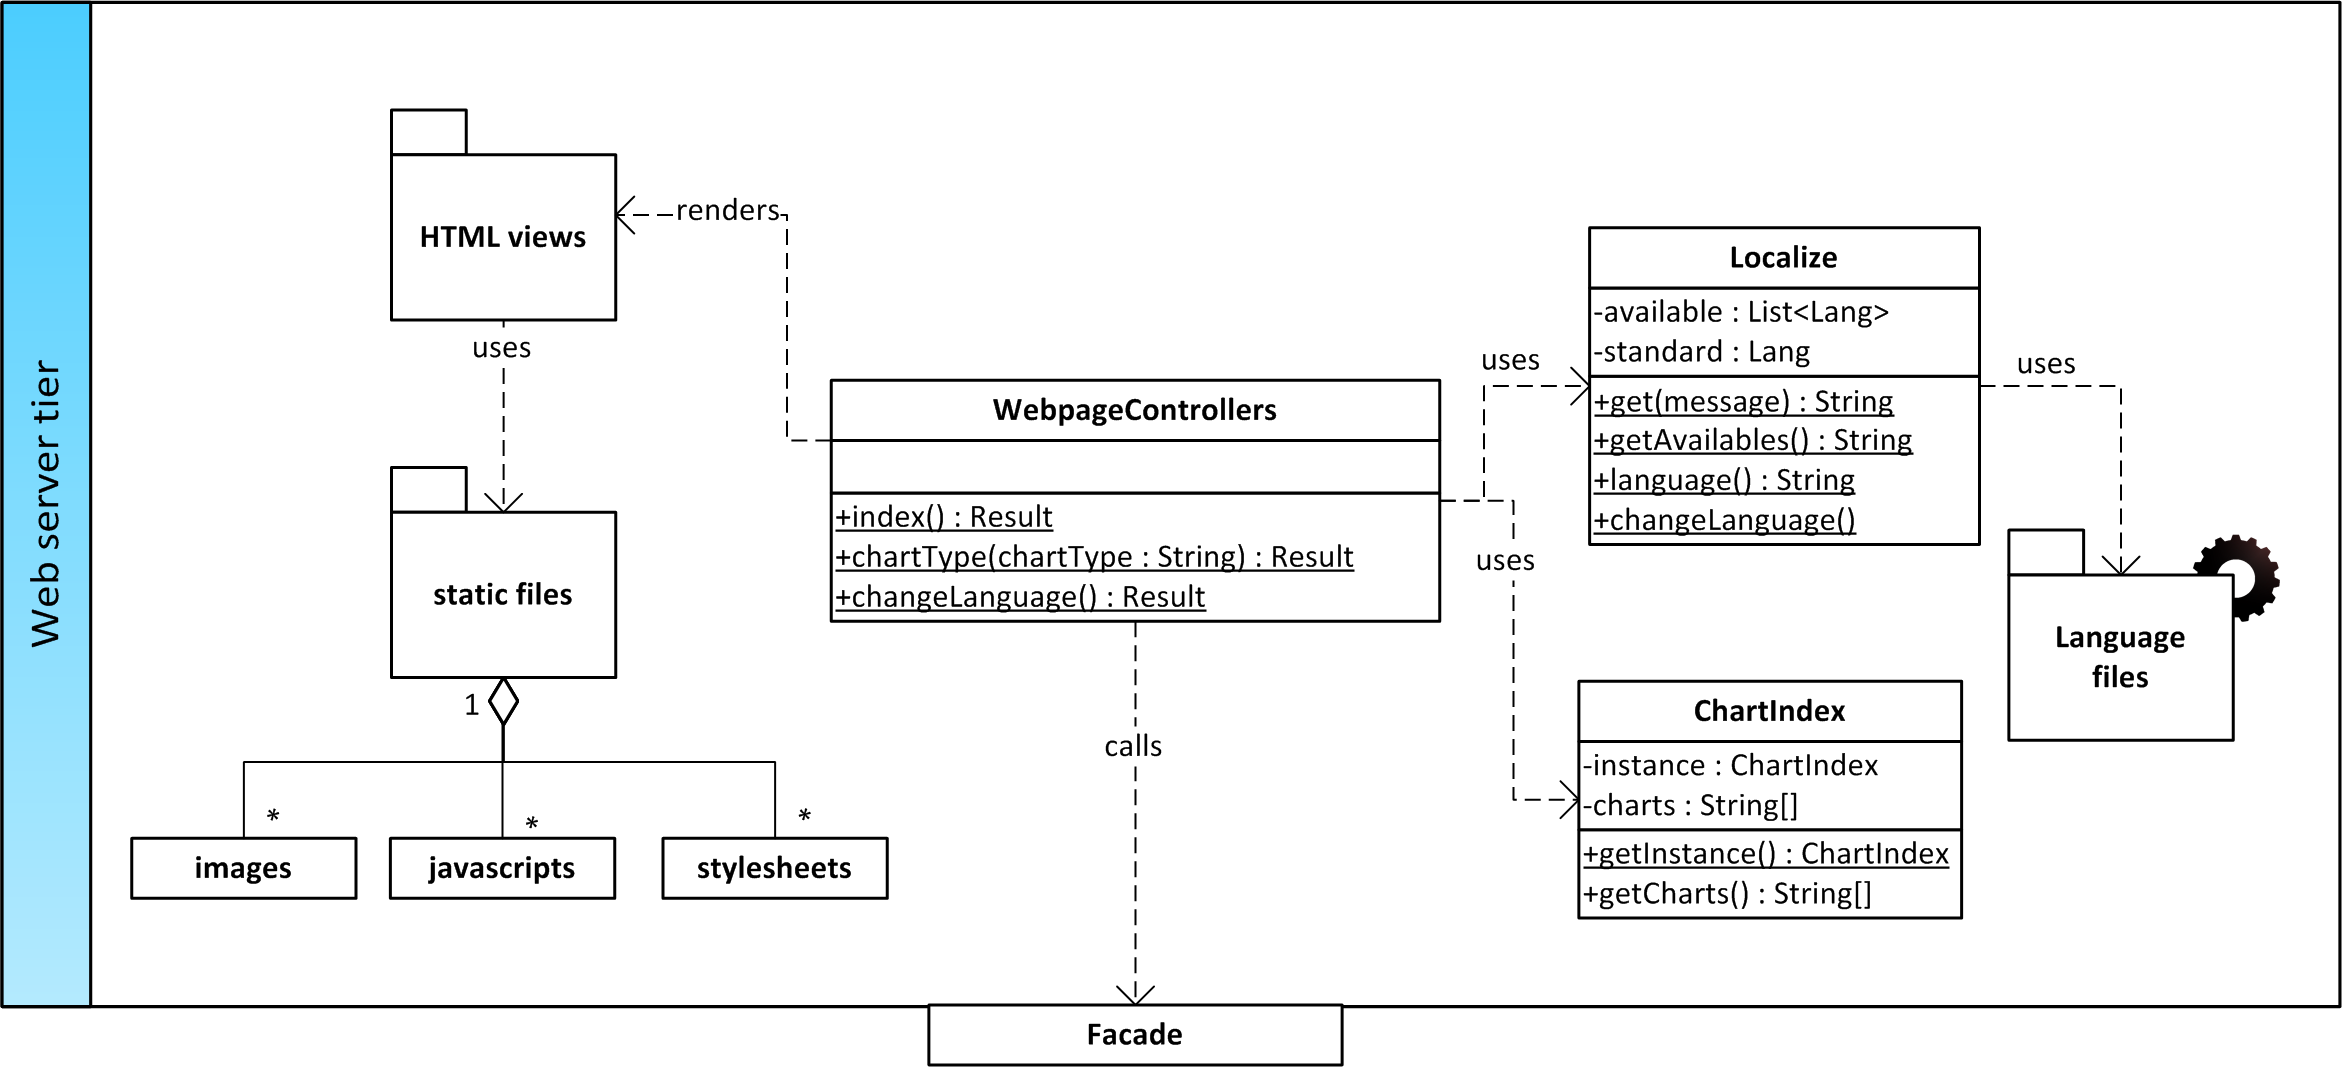
\includegraphics[width=1\linewidth]{Pictures/ServerTierDiaNormal.png} 
\end{center}   


\subsubsection*{WebpageControllers}
All valid HTTP requests are mapped to a method from WebpageControllers.
WebpageControllers either uses other helper classes to handle requests itself  
or makes calls to the facade of the application tier. 
The last step done by WebpageControllers is to create a valid HTTP response.
                                                                            

\subsubsection*{HTML views}
The HTML views contain the main template for, and all other HTML content of the web page. %unklar
They do not have to be static, but can also dynamically integrate some content, e.g. localized strings.

\subsubsection*{Static files}
Static files contains all files of the web page, which are not changed during runtime. 
This includes, but is not limited, to images of the web page, javascript files and stylesheets.

\subsubsection*{Localize}
Localize is a static helper class handling all the language related things. 
It has a method to get localized Strings using the language files, 
to change the language of the web page und methods determining all available languages, 
%dieser Satz, passt der syntaktisch? Sollte es methods sein?
so they can be integrated in the web page once they are present.

\subsubsection*{ChartIndex}
ChartIndex implements the singleton pattern. On instantiation it scans which chart types are available 
and saves them internally. This is used by the index page to dynamically display all available chart types,
even if one is deleted or added.
%Do we have to specify how one might add them? I mean, not here, but somewhere.


%=||======================================================================>
\subsection{Application \& Data access tier class diagram}
On the next pages the class diagram of the application and data access tier are displayed. 
\newpage
\begin{center}
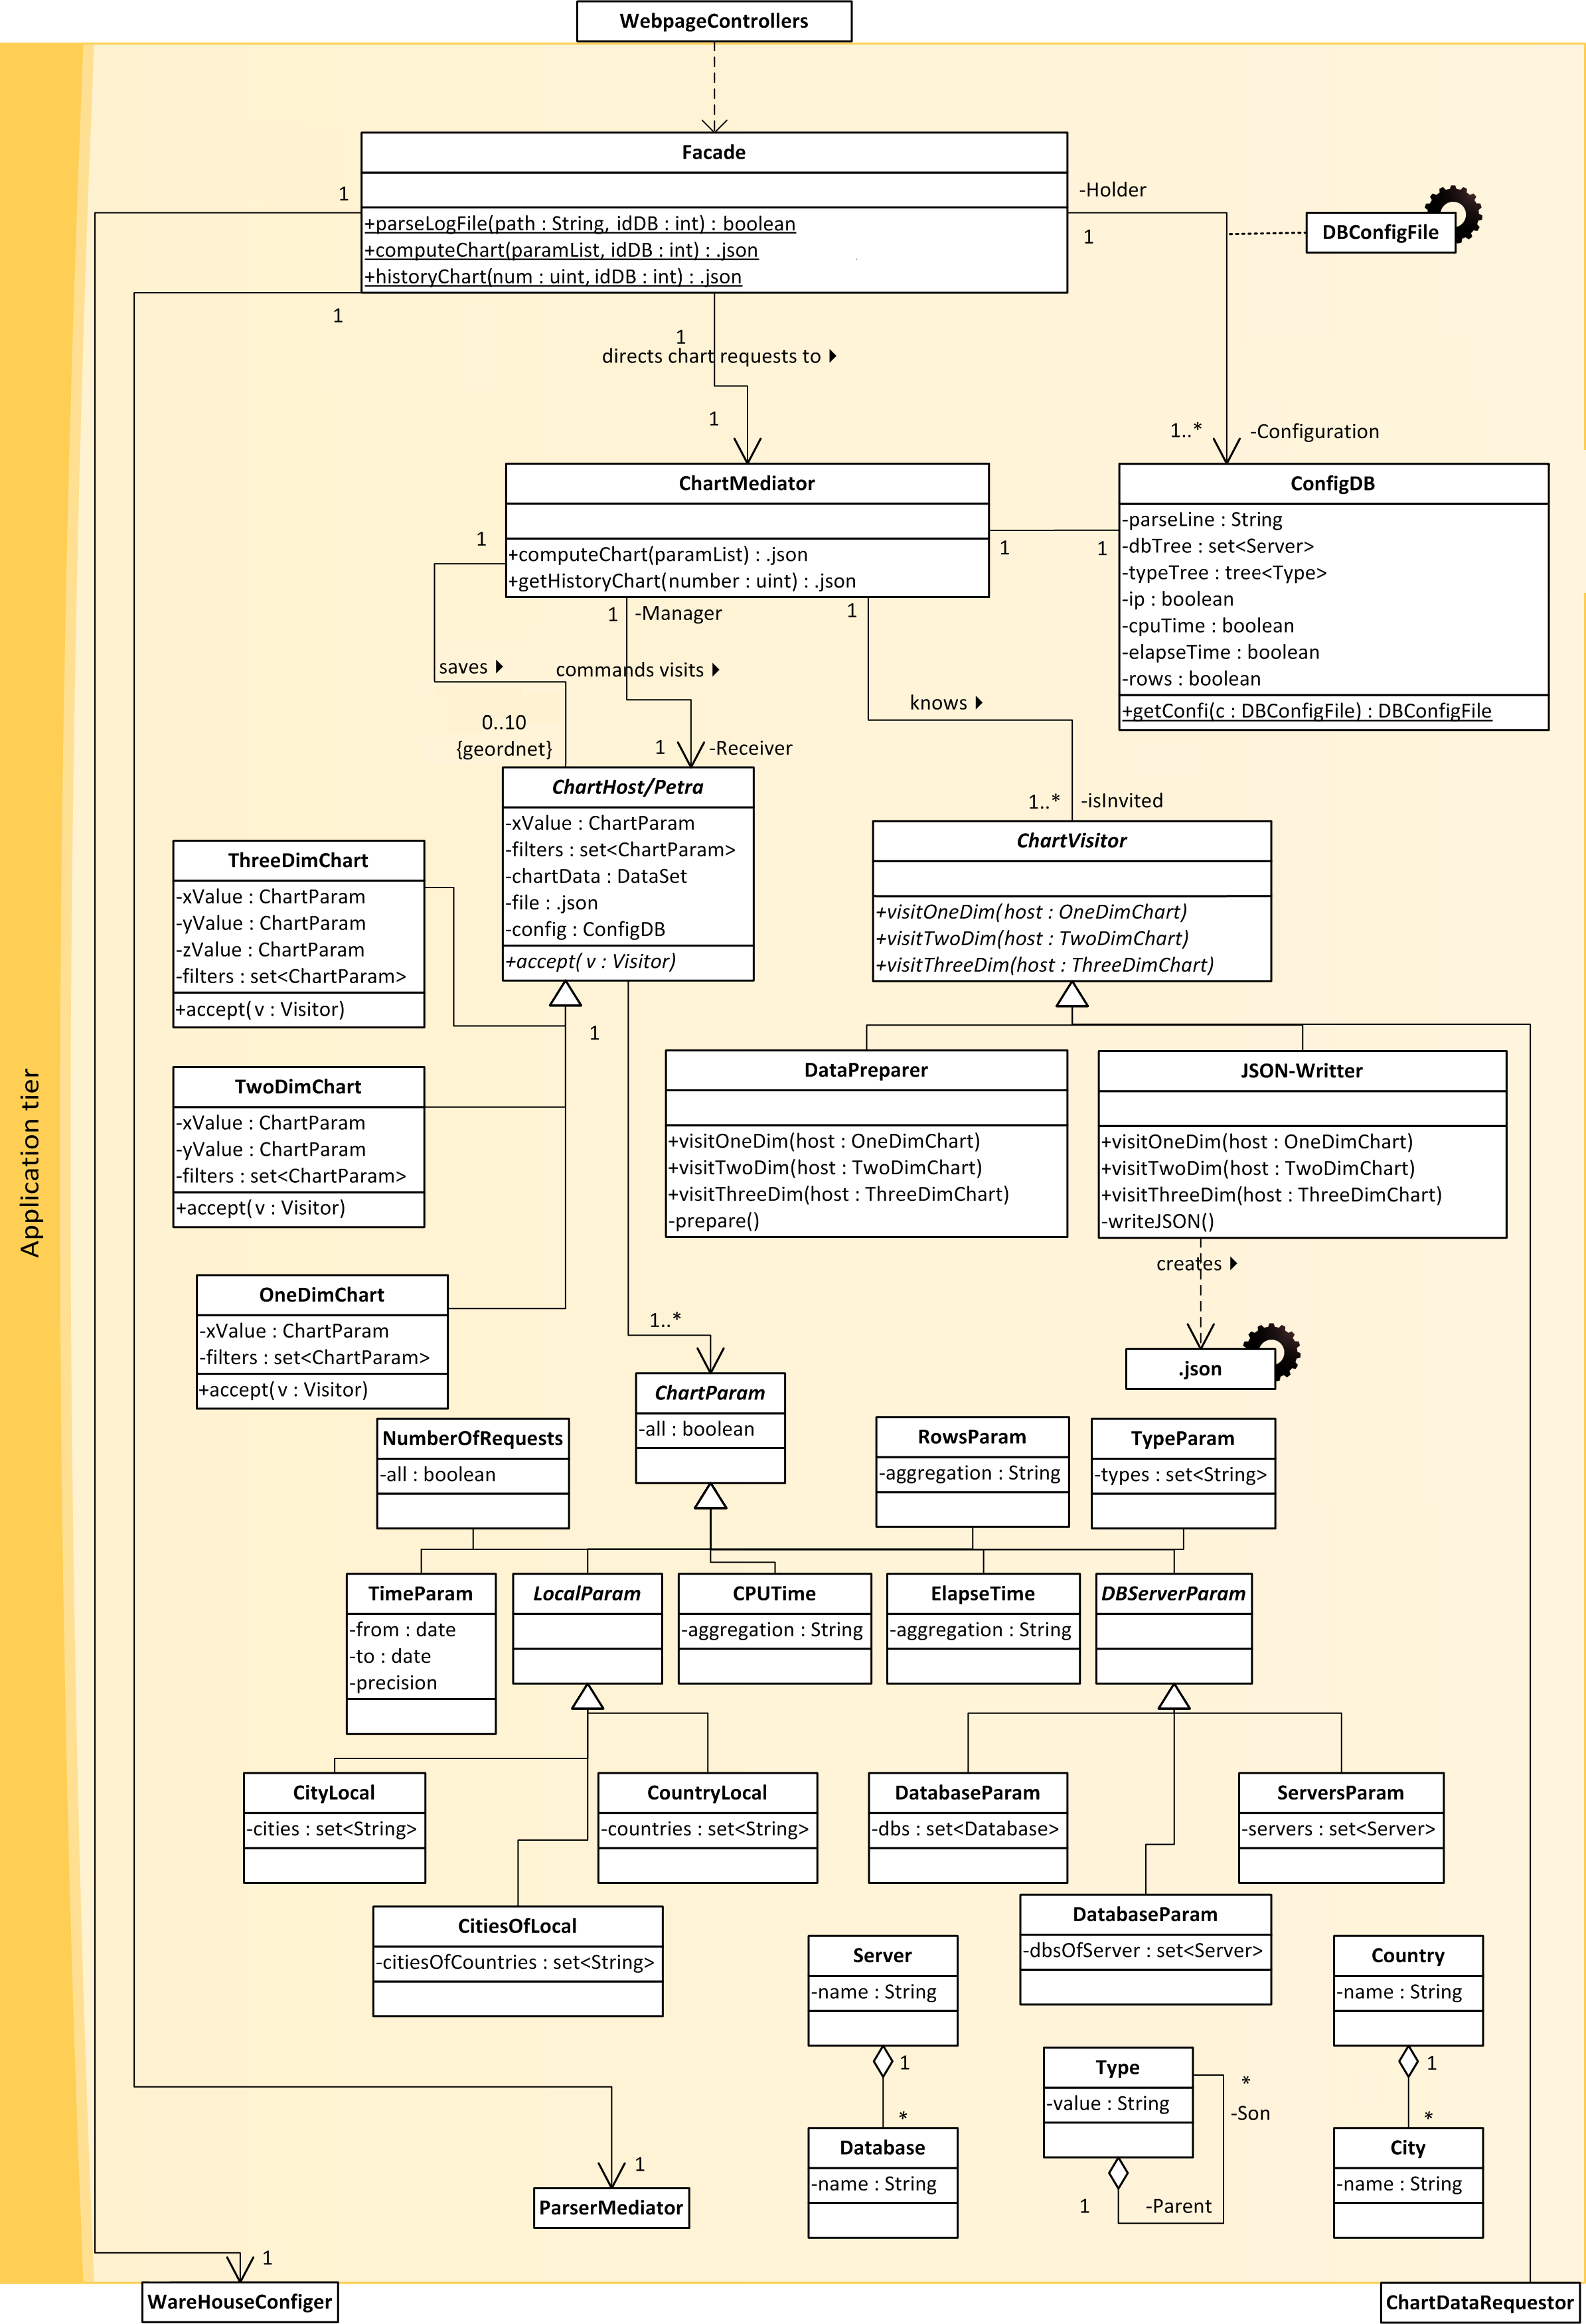
\includegraphics[width=0.9\linewidth]{Pictures/AppTierDia1.png}
%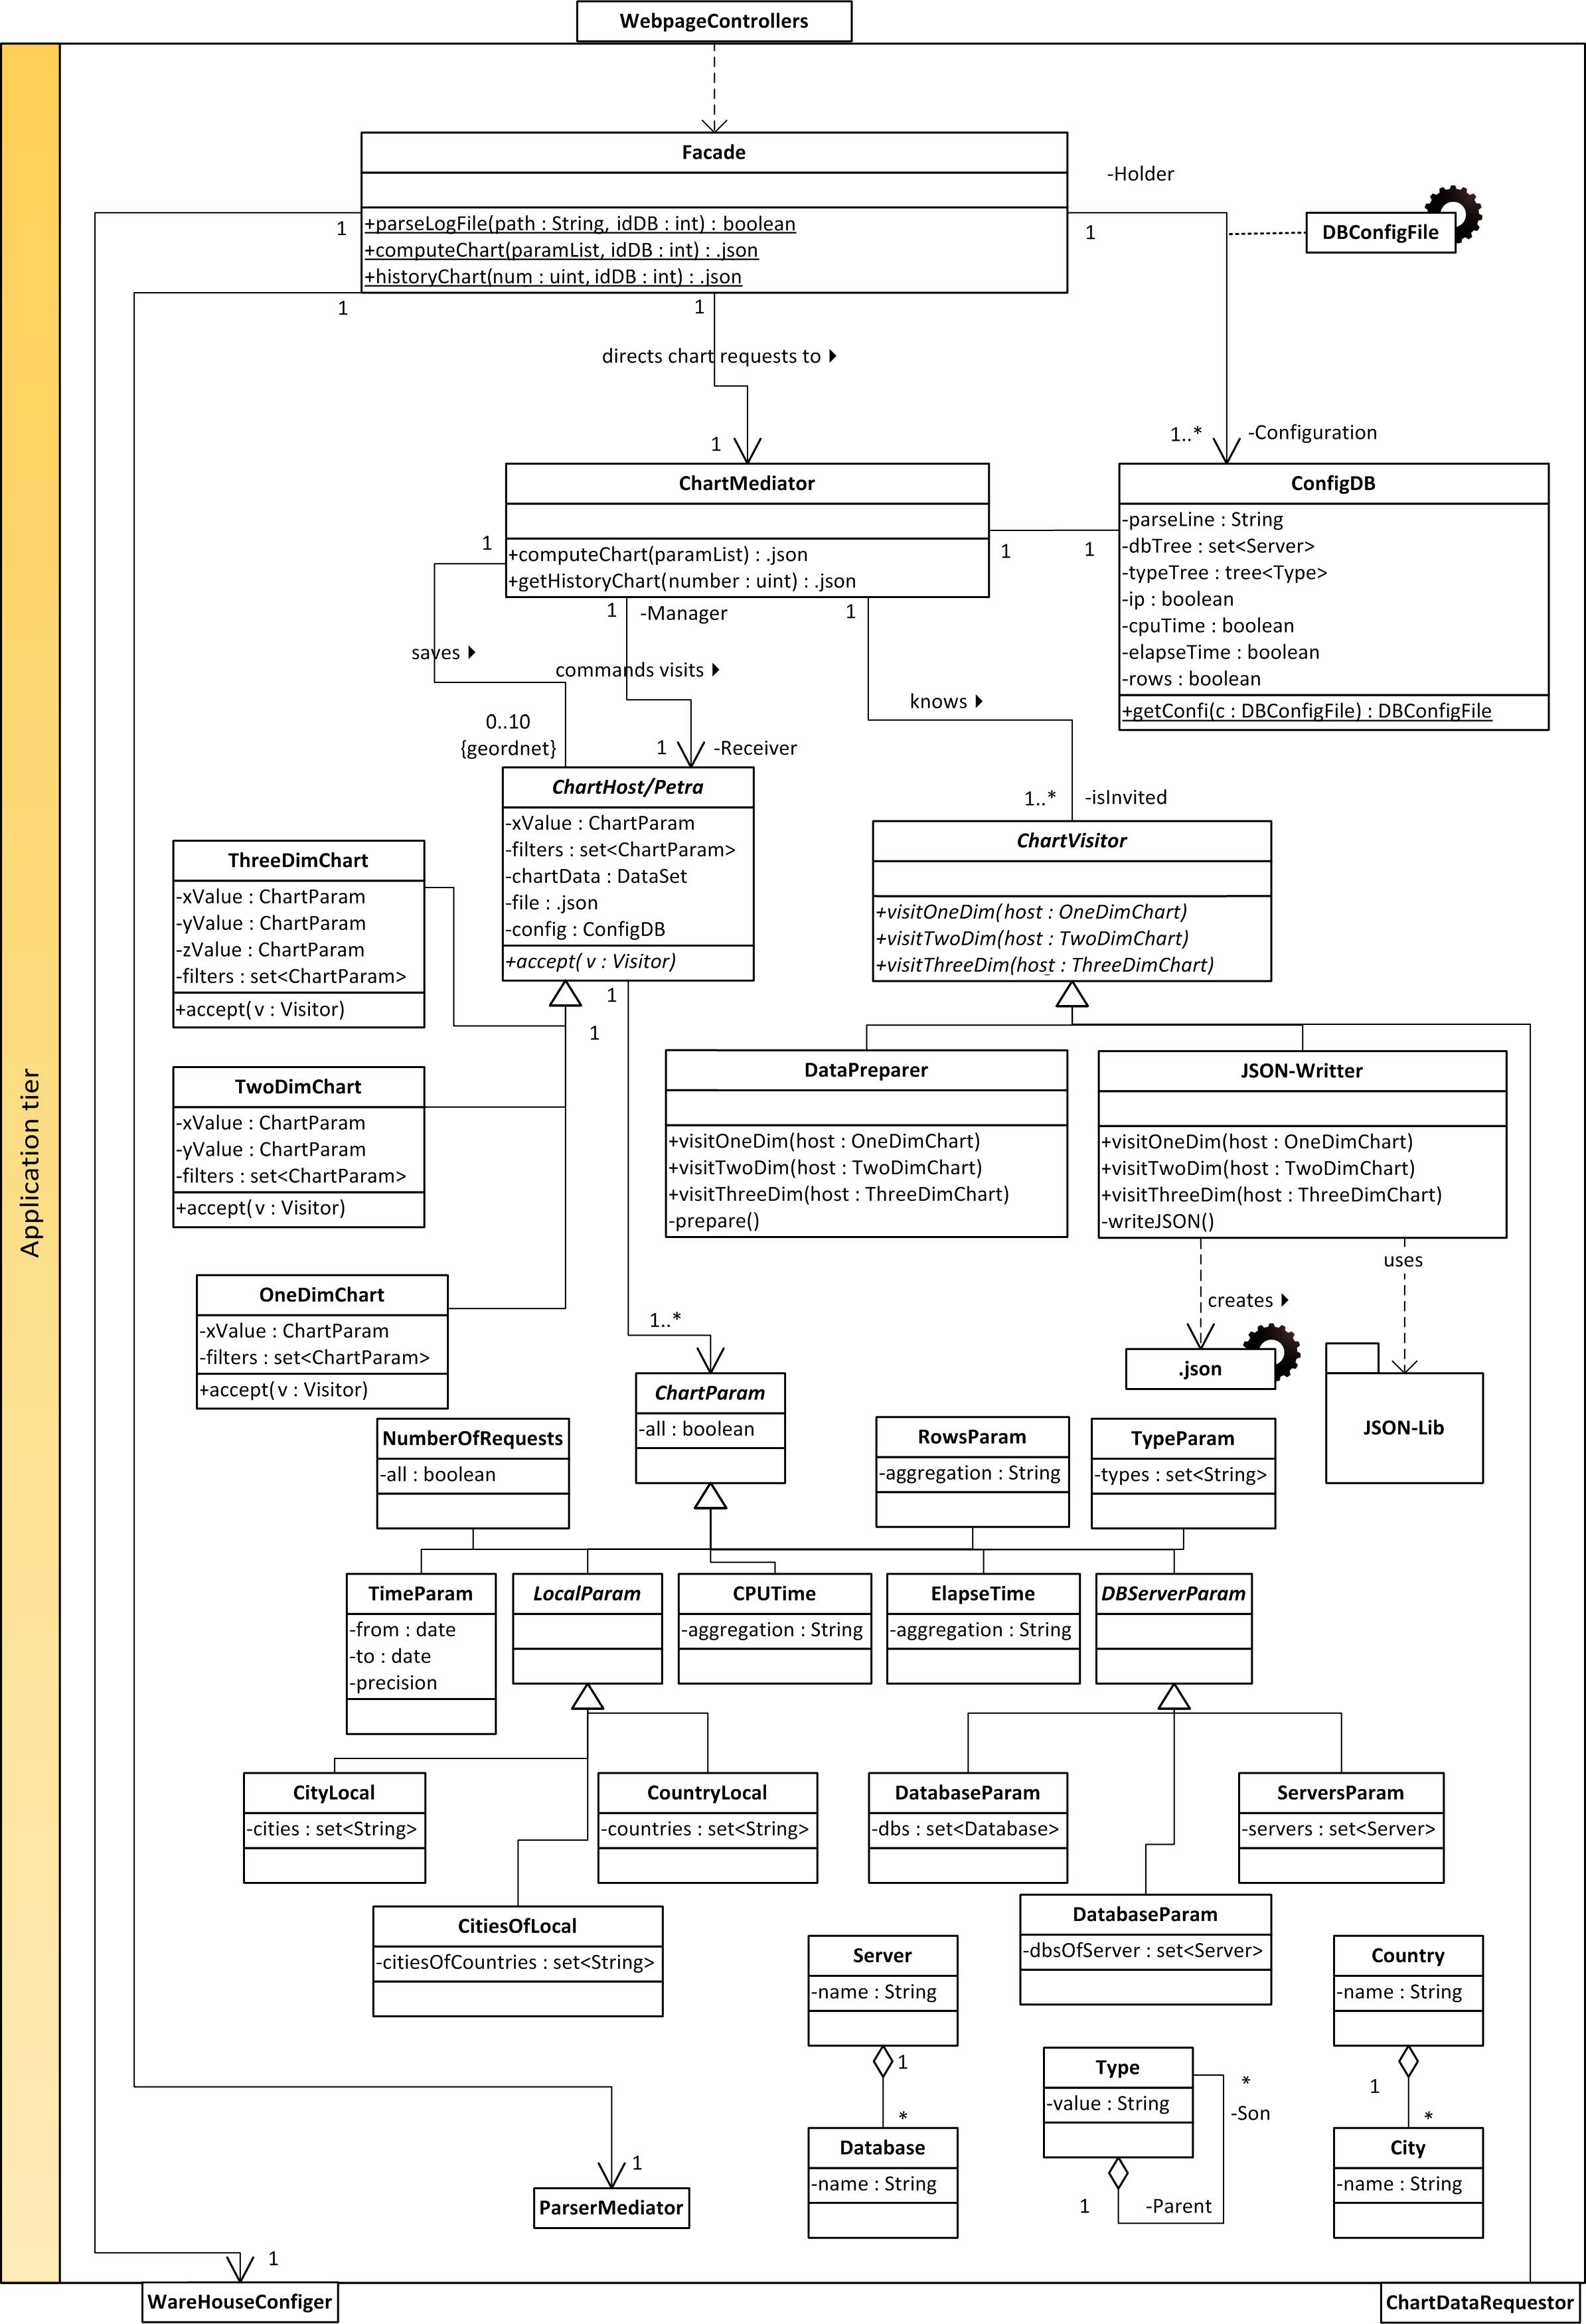
\includegraphics[width=0.9\linewidth]{Pictures/AppTierDia1Normal.png} 
\end{center}  

\begin{center}
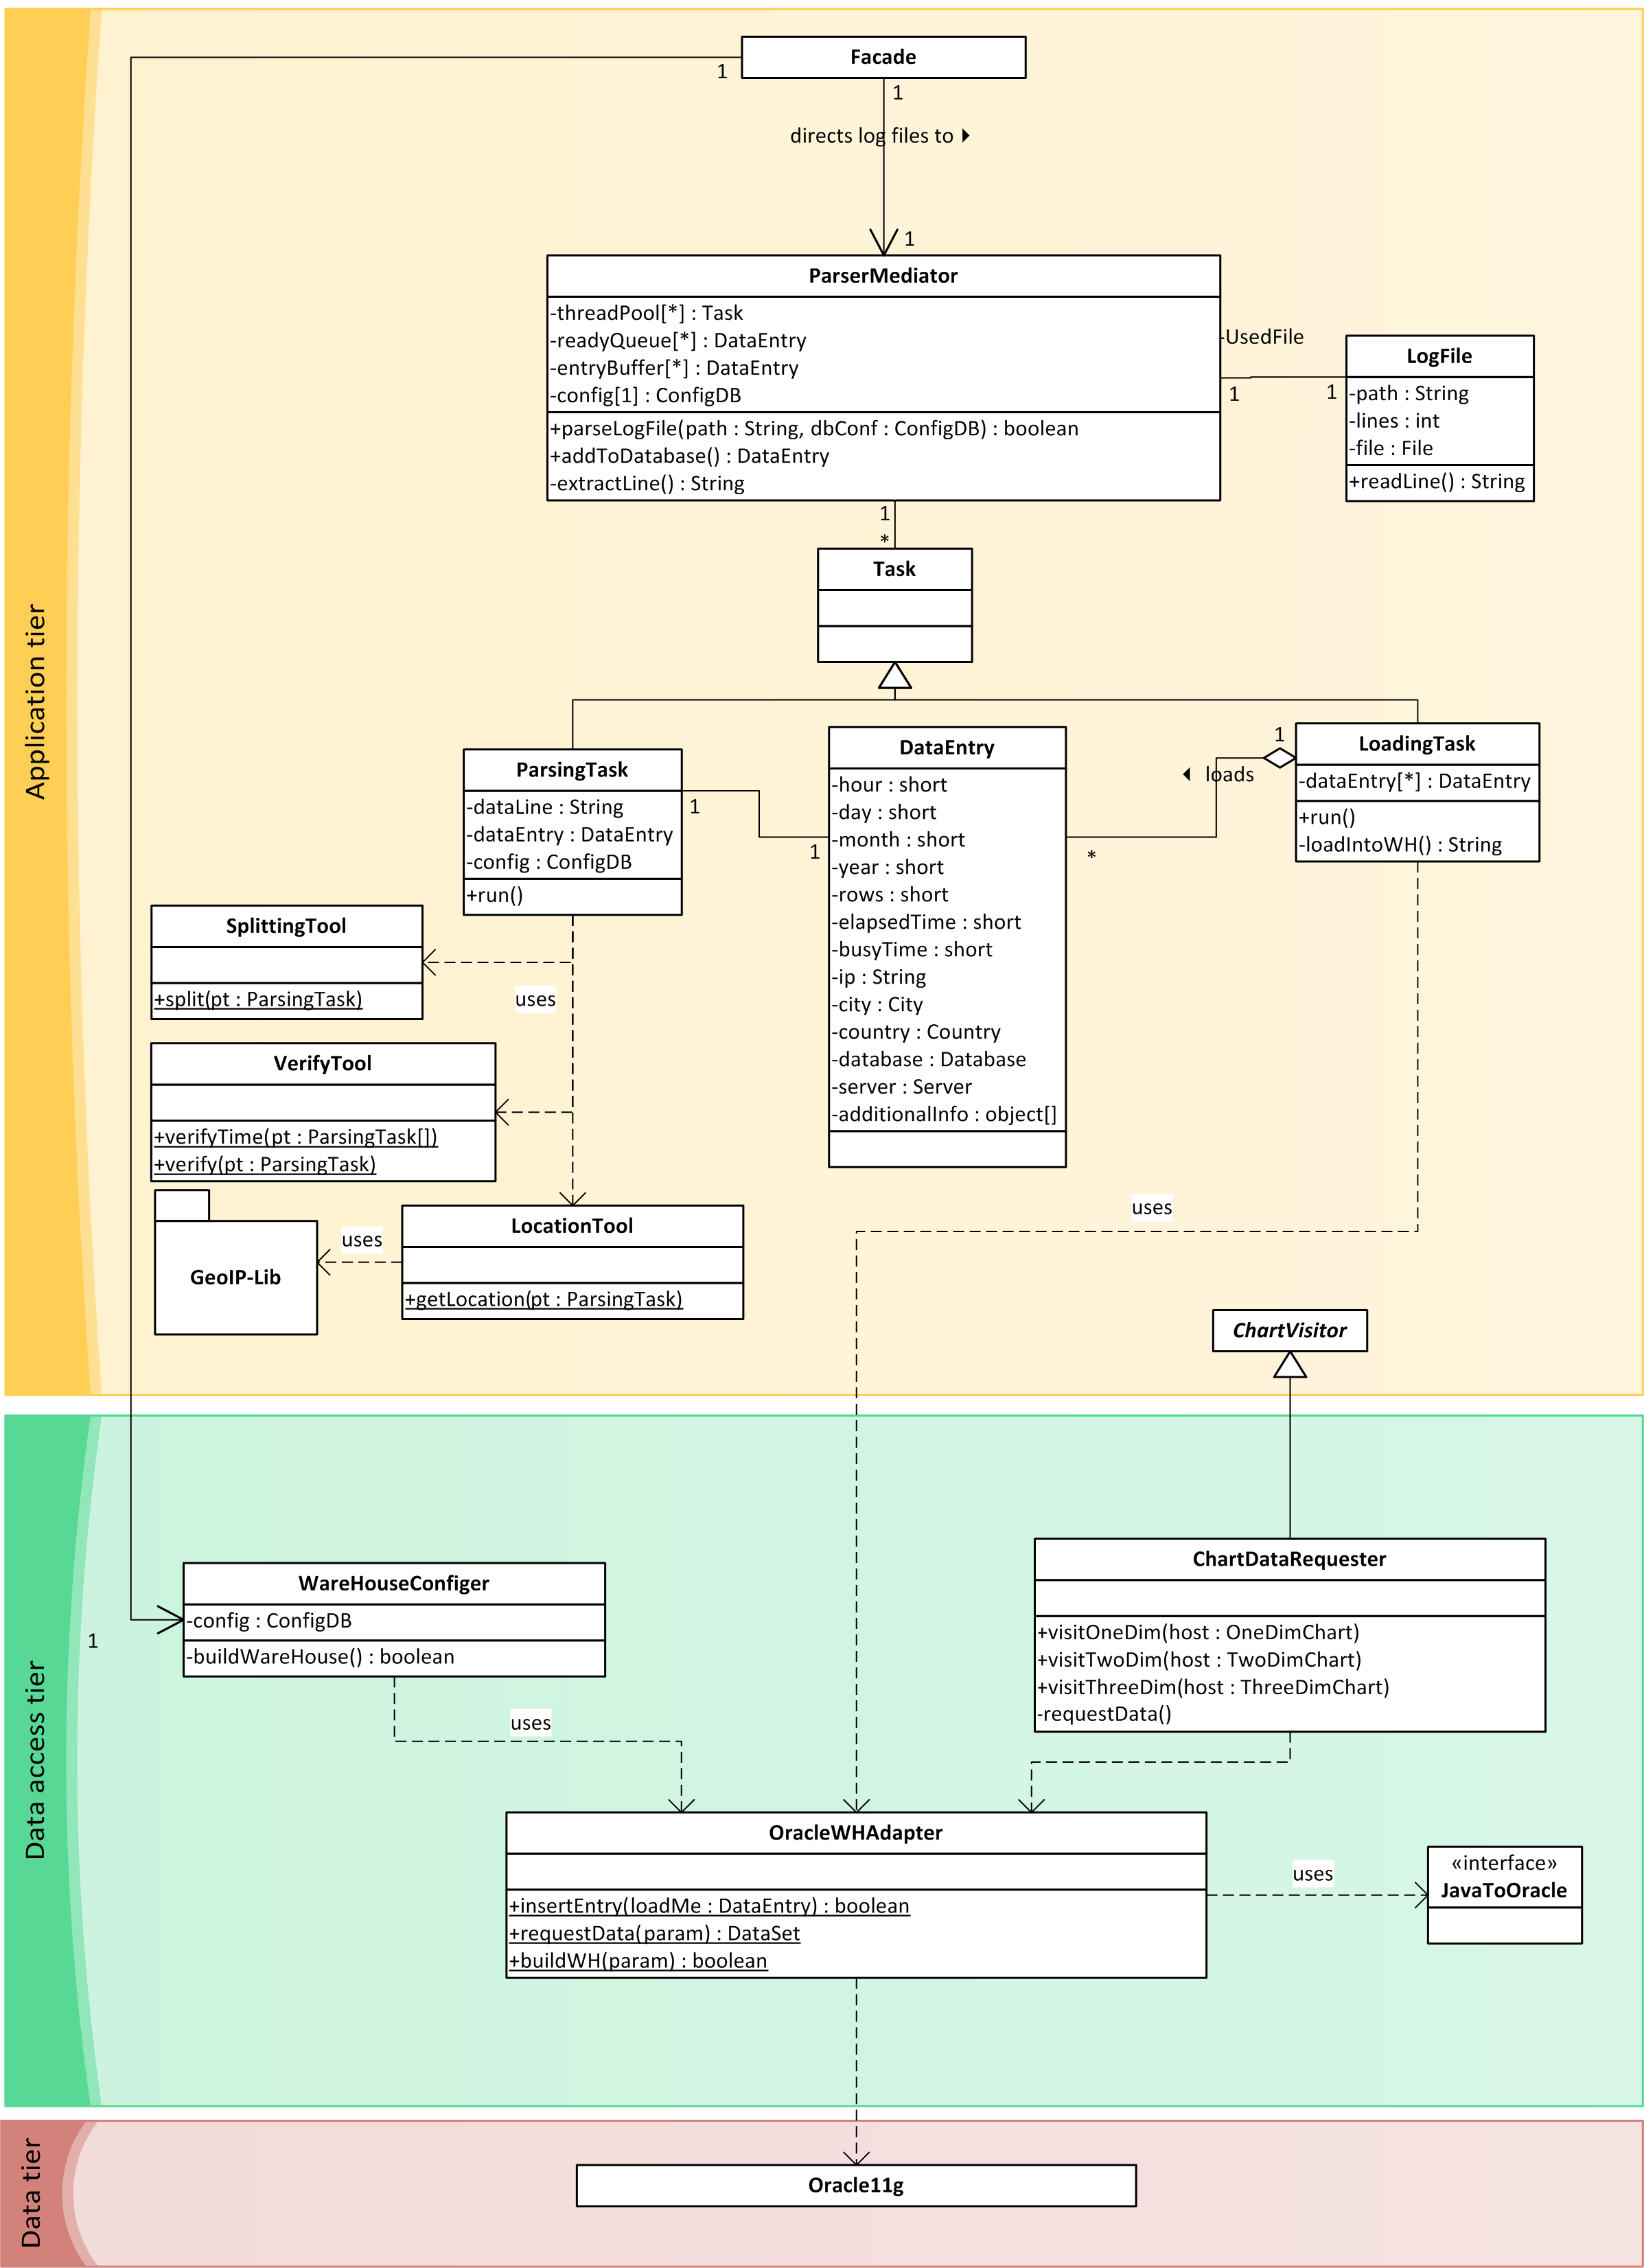
\includegraphics[width=0.9\linewidth]{Pictures/AppTierDia2.png}
%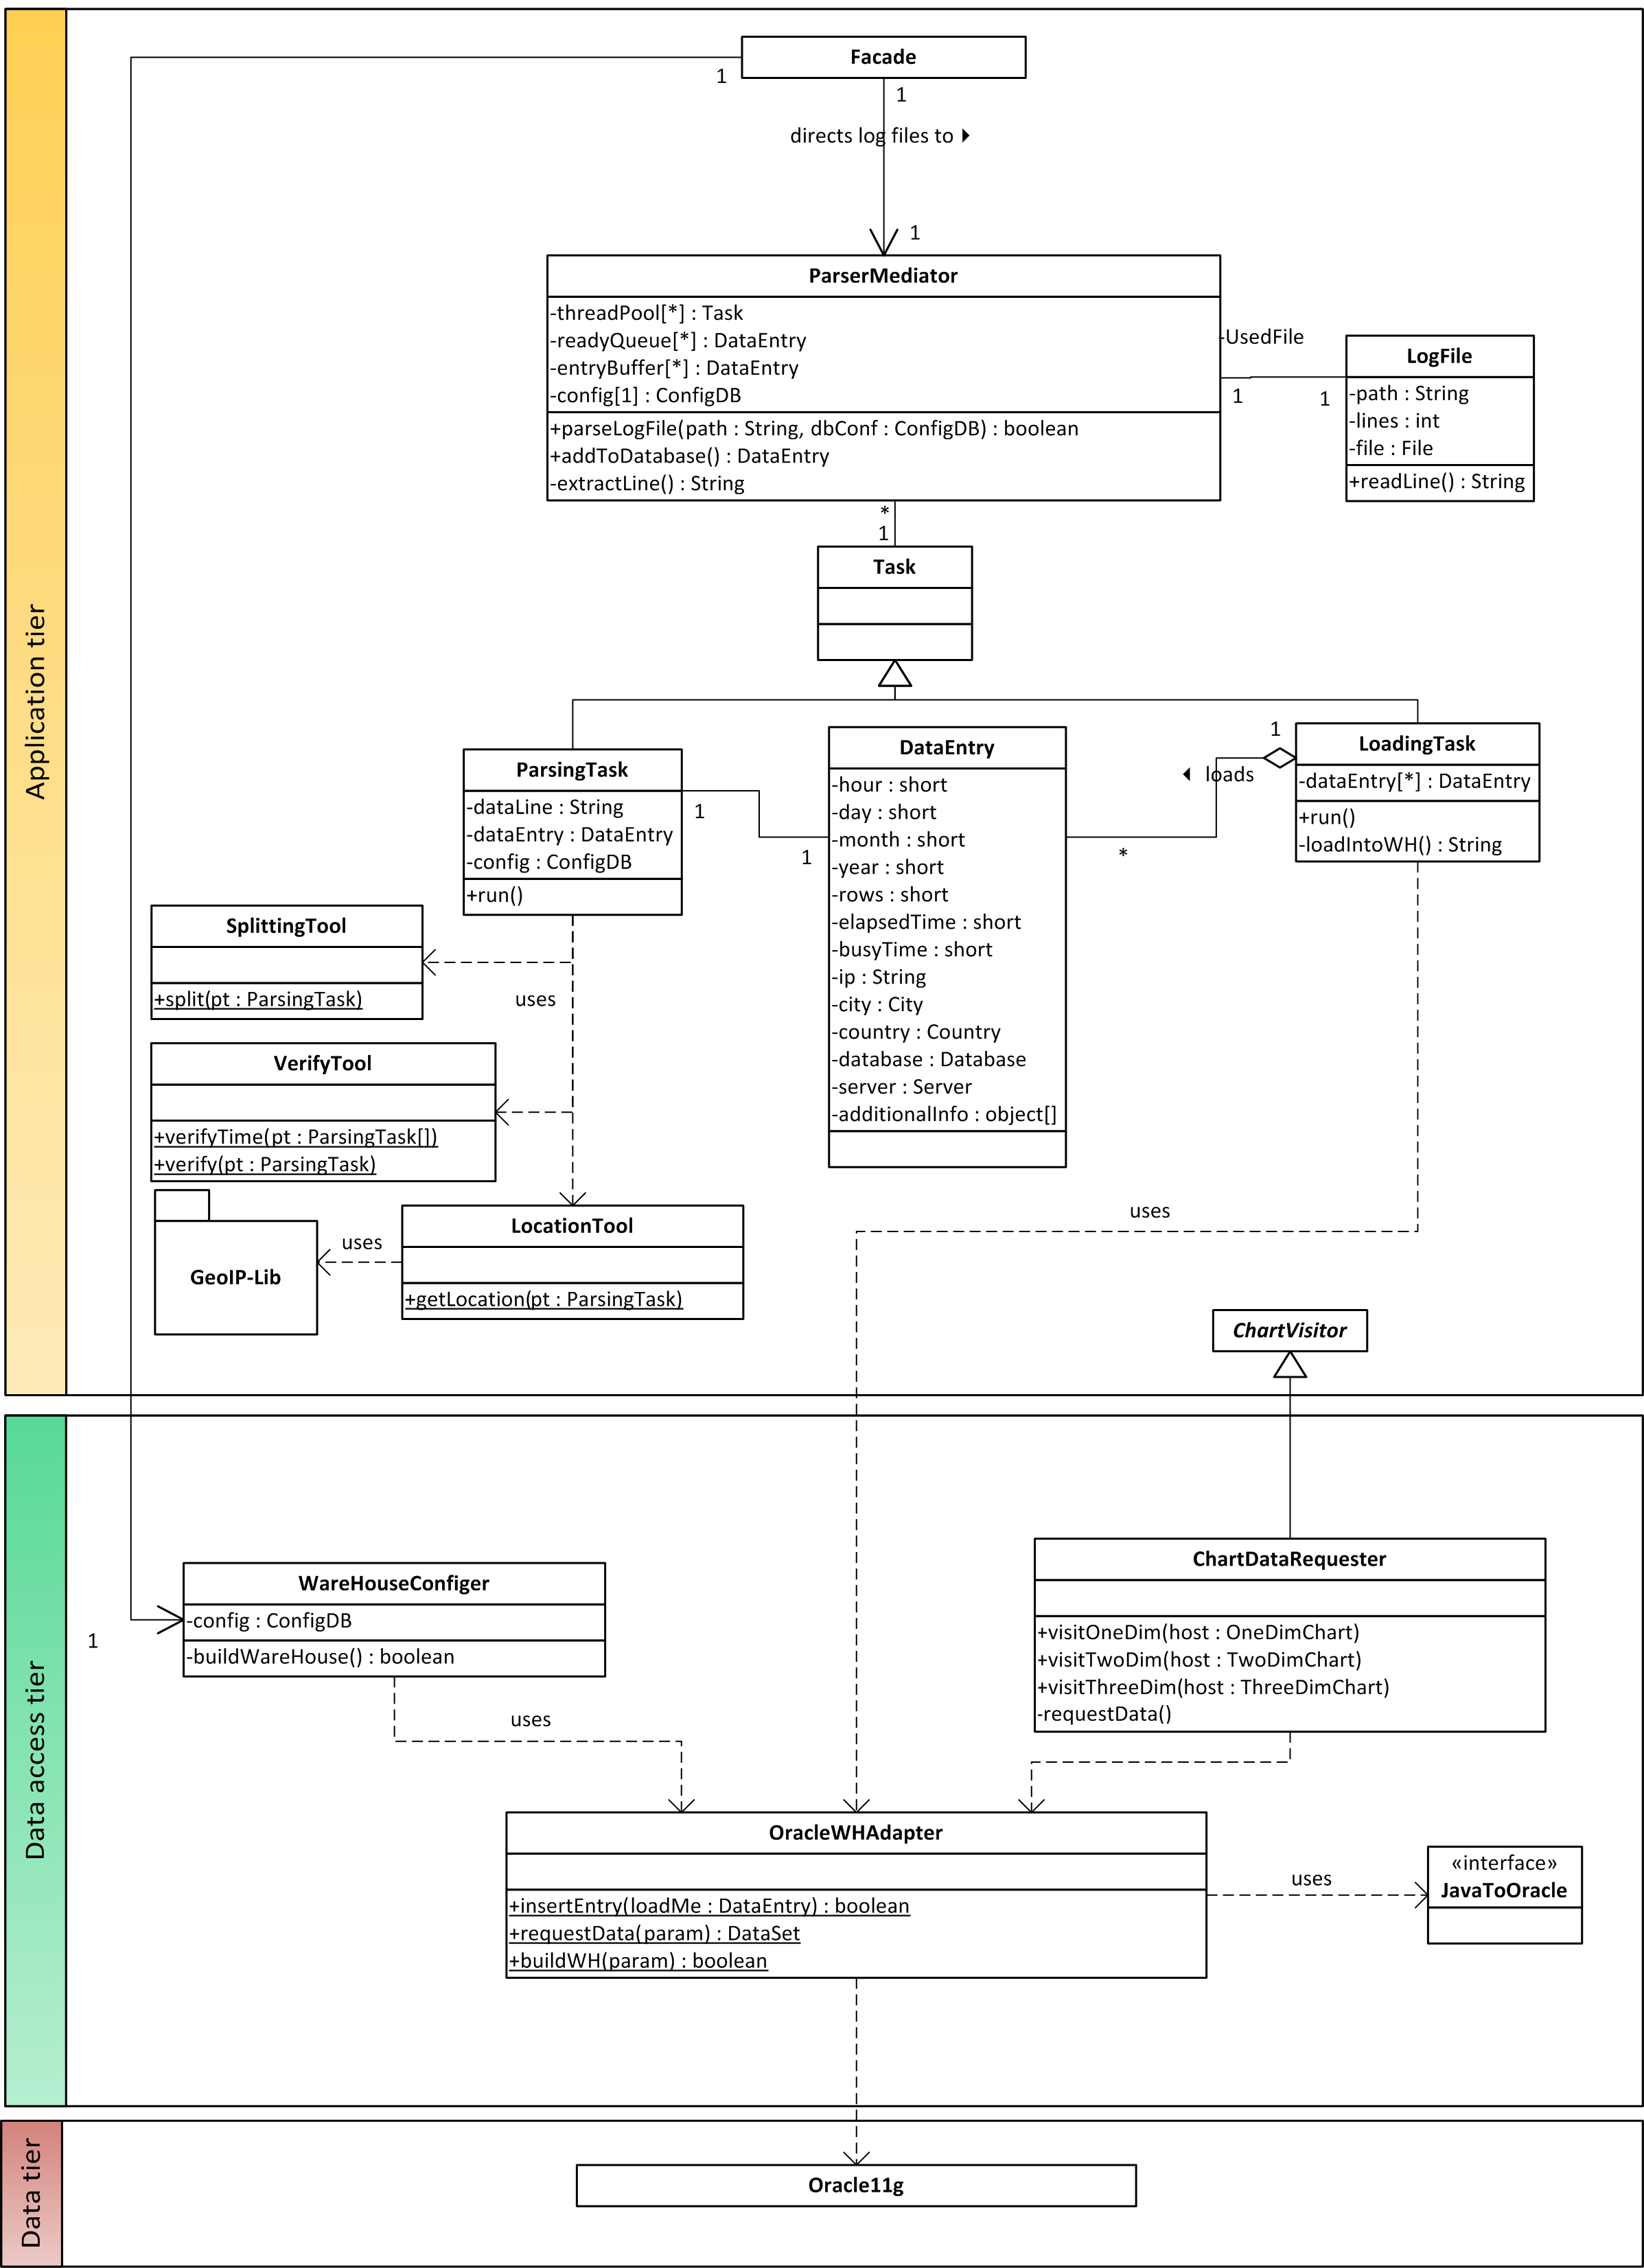
\includegraphics[width=0.9\linewidth]{Pictures/AppTierDia2Normal.png} 
\end{center}  

%=||======================================================================>
\subsection{Facade + Configurations}
The facade of the application tier and configuration files in this design show a
optional feature. According to the database on which is operated - if there are more
than SkyServer - just a configuration file for this specific one, has to be created and
given to the program. This may give the application the power to manage all functions dynamically
according to the database. Facade and ConfigDB handle this configurations.


\begin{center}
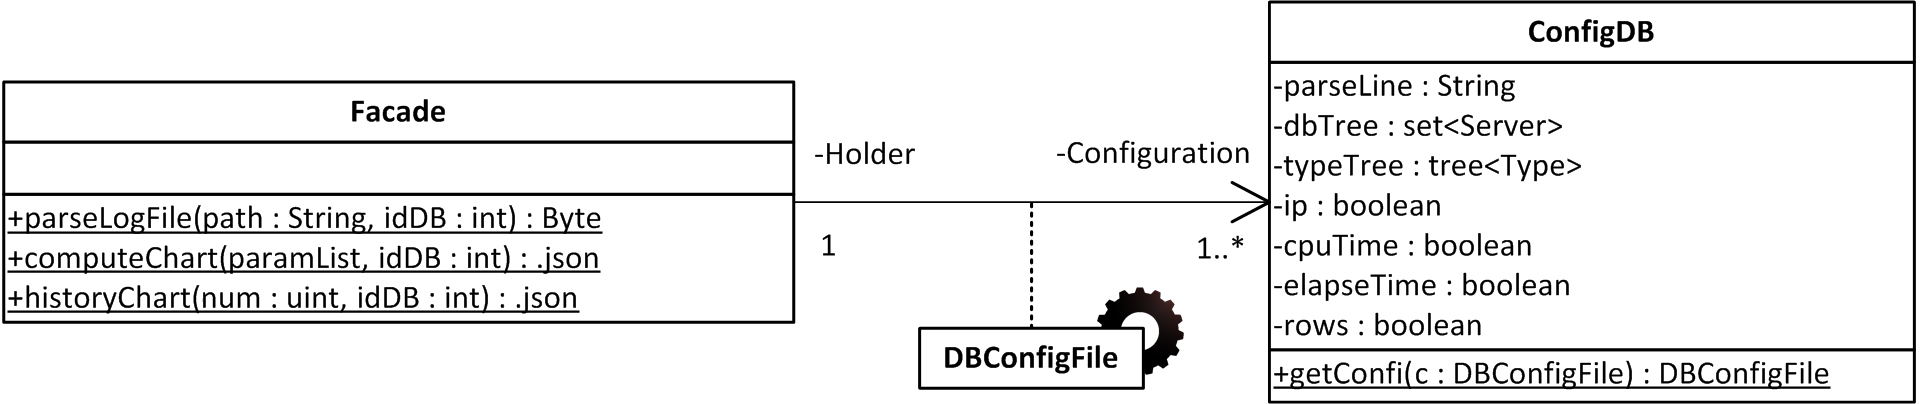
\includegraphics{Pictures/Parts/FacadeConfi.png}
\end{center}   

\subsubsection*{Facade}
The Facade is, as you might have suggested, the facade of the application tier. 
This means the only way to communicate with this tier is via this class.
One of its tasks is to get the right ConfigDB for any call. With this it forwards
them to the corresponding mediators or workers. So new log files are passed to
the ParserMediator and chart requests to the ChartMediator. Some other optional
calls, like the history of charts or the configuration of a new warehouse are just
adumbrated. %nice word wtf :D no one will know it


\subsubsection*{ConfigDB}
The ConfigDB class provides a static factory for creating itself out of a configuration
file, which may use caching. Objects of ConfigDB store the information about the database
they describe and will be used by all the dynamic methods, which are hooked on specific
databases. 

One thing stored in a ConfigDB is a String indicating the form of a line in the log files.
Other attributes are booleans for specific measures or dimensions, as well as trees of
Strings for dimensions like Database > Server or the Type.

\newpage
\begin{center}
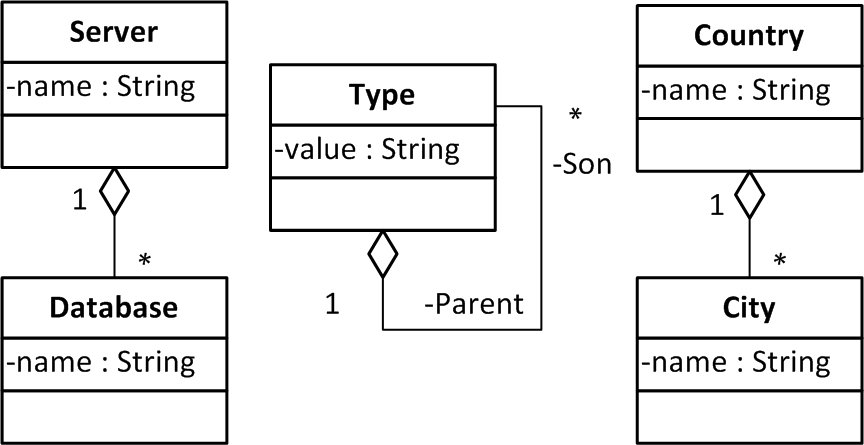
\includegraphics{Pictures/Parts/Strings.png}
\end{center}  
\subsubsection*{Server, Database, Type, Country, City}
All this classes are Stringwrappers and also build as trees. They stand exemplary for
possible things stored in a ConfigDB. The implementation of them may be way more dynamic.
Whereas the content of Server \& Database and Type are depended on the configuration,
the Country \& City tree is mostly hooked to the GeoIP library.


%=||======================================================================>
\subsection{Chart request operator}
The task of the following classes is to handle a chart request. For their design the visitor pattern
is used. 

\begin{center}
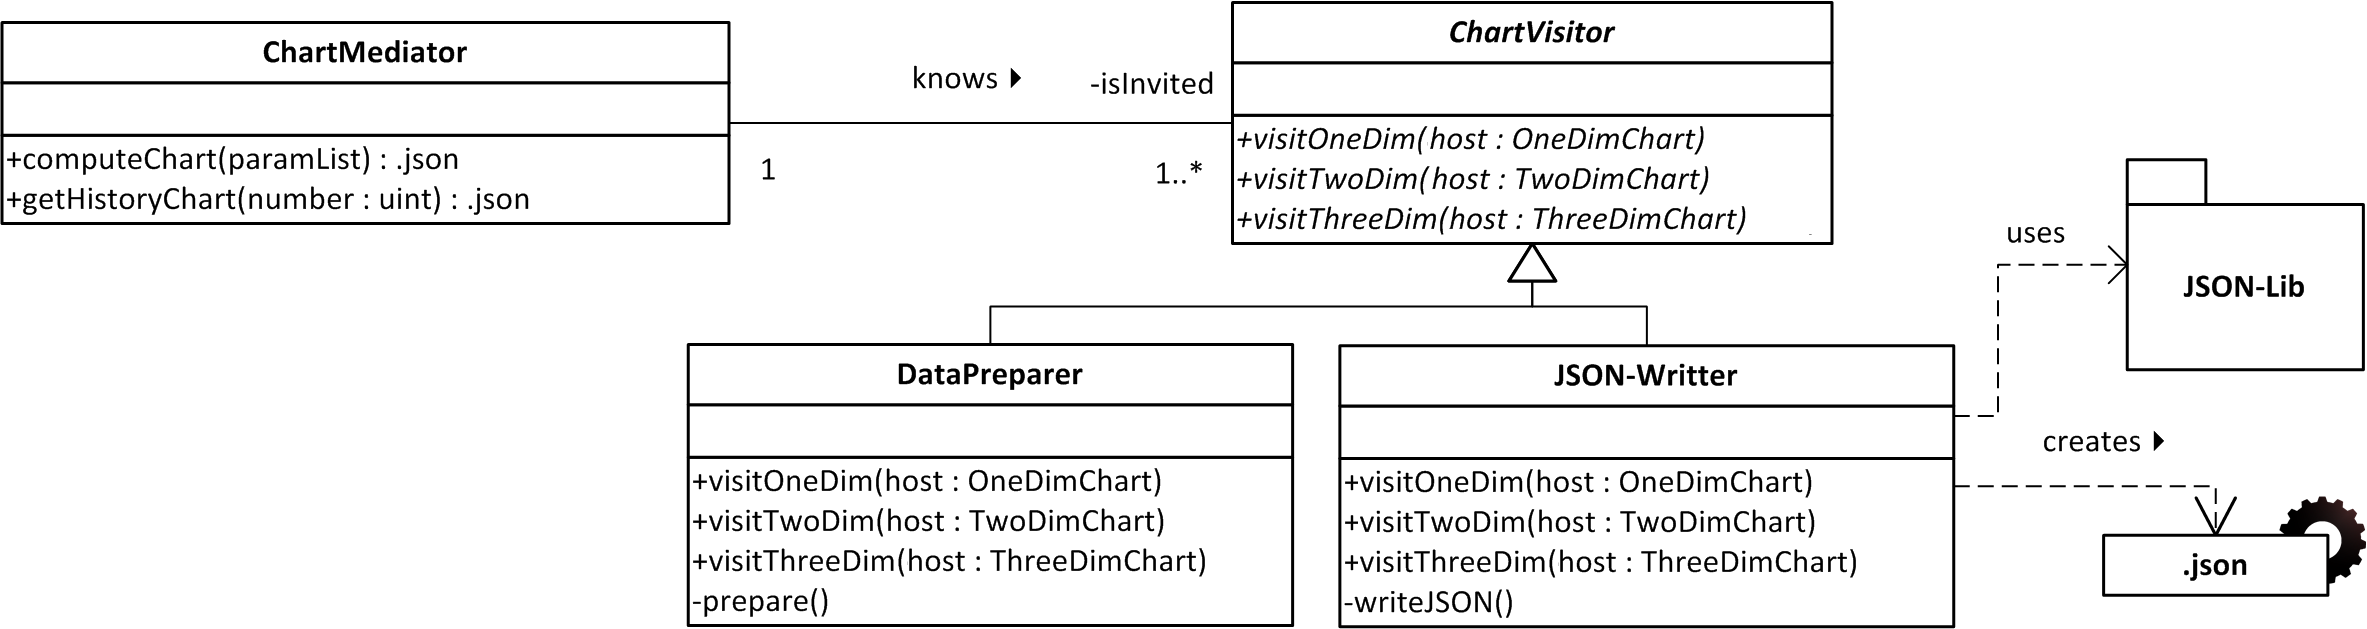
\includegraphics[width=1\linewidth]{Pictures/Parts/MediVisi.png}
\end{center}  

\subsubsection*{ChartMediator}
The ChartMediator is the mediator of the whole chart request process. For a incoming request it will create a new
ChartHost firstly. Then it triggers the visits of the three visitors. 


\subsubsection*{ChartVisitor}
ChartVisitors work on a ChartHost. What the visitors do depends on which specific ChartHost 
is visited and of course on their type. 
One visitor, the ChartDataRequester, is part of the data access tier.


\subsubsection*{DataPreparer}
The DataPreparer is the second visitor. It prepares the raw data stored in a ChartHost, so that the JSON-Writter
can do its work easily.


\subsubsection*{JSON-Writter}
The JSON-Writter is the last visitor. According to the data stored in the visited ChartHost he creates a .json file
which contains all information needed by D3 to display the charts. 

\begin{center}
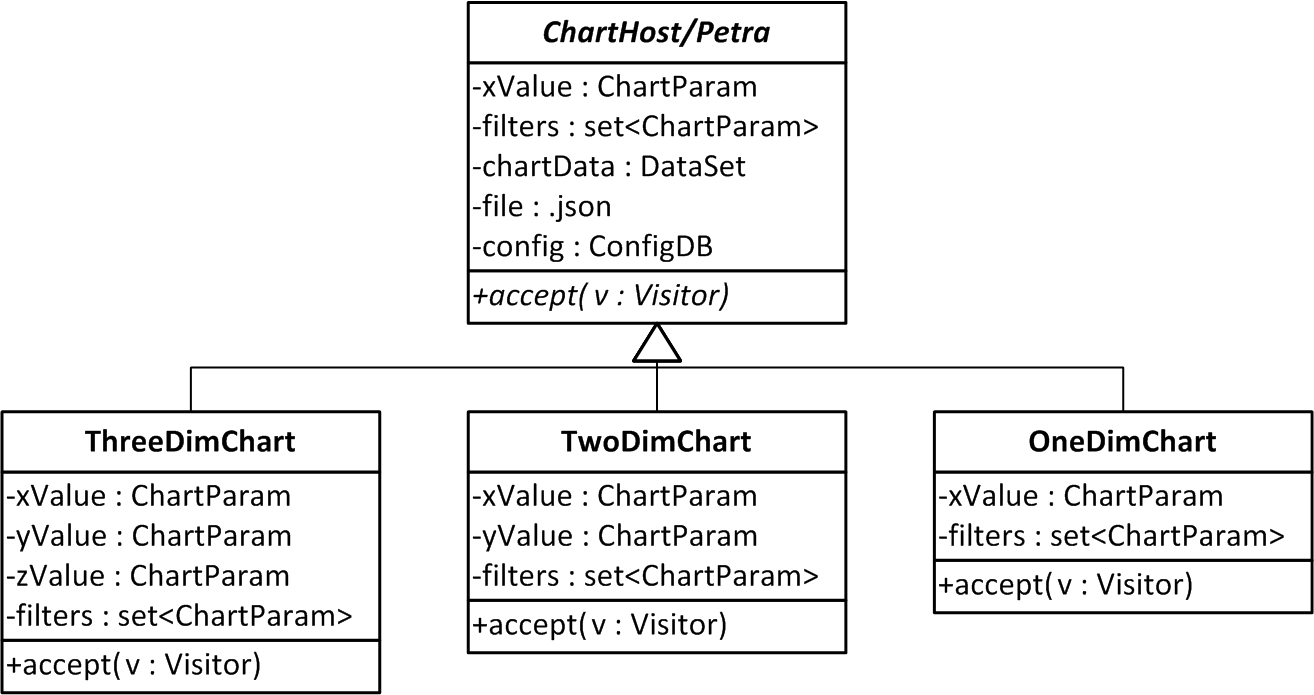
\includegraphics{Pictures/Parts/Petra.png}
\end{center}  

\subsubsection*{ChartHost/Petra}
ChartHosts are objects hosting one chart request. Once initialized, they store the chart parameteres requested for
the axes and the filter options. During the visits they first store raw data and later the .json file needed
for the chart.
The other name Petra for ChartHost is the intern name used for this class. As it had no official name it was
and still is known by Petra. So because when mentioning Petra all current members know what is meant the name
is also given in this design document.

\subsubsection*{OneDimChart}
A OneDimChart - the name standing for one dimension chart - stores the ChartParam for the x axes or for example
just the measure/radius needed in a bubble chart.
 
 
\subsubsection*{TwoDimChart}
More than the OneDimeChart the TwoDimChart also stores the ChartParam of a second axis.

\subsubsection*{ThreeDimChart} 
The ThreeDimChart stores ChartParams for three axes.

\begin{center}
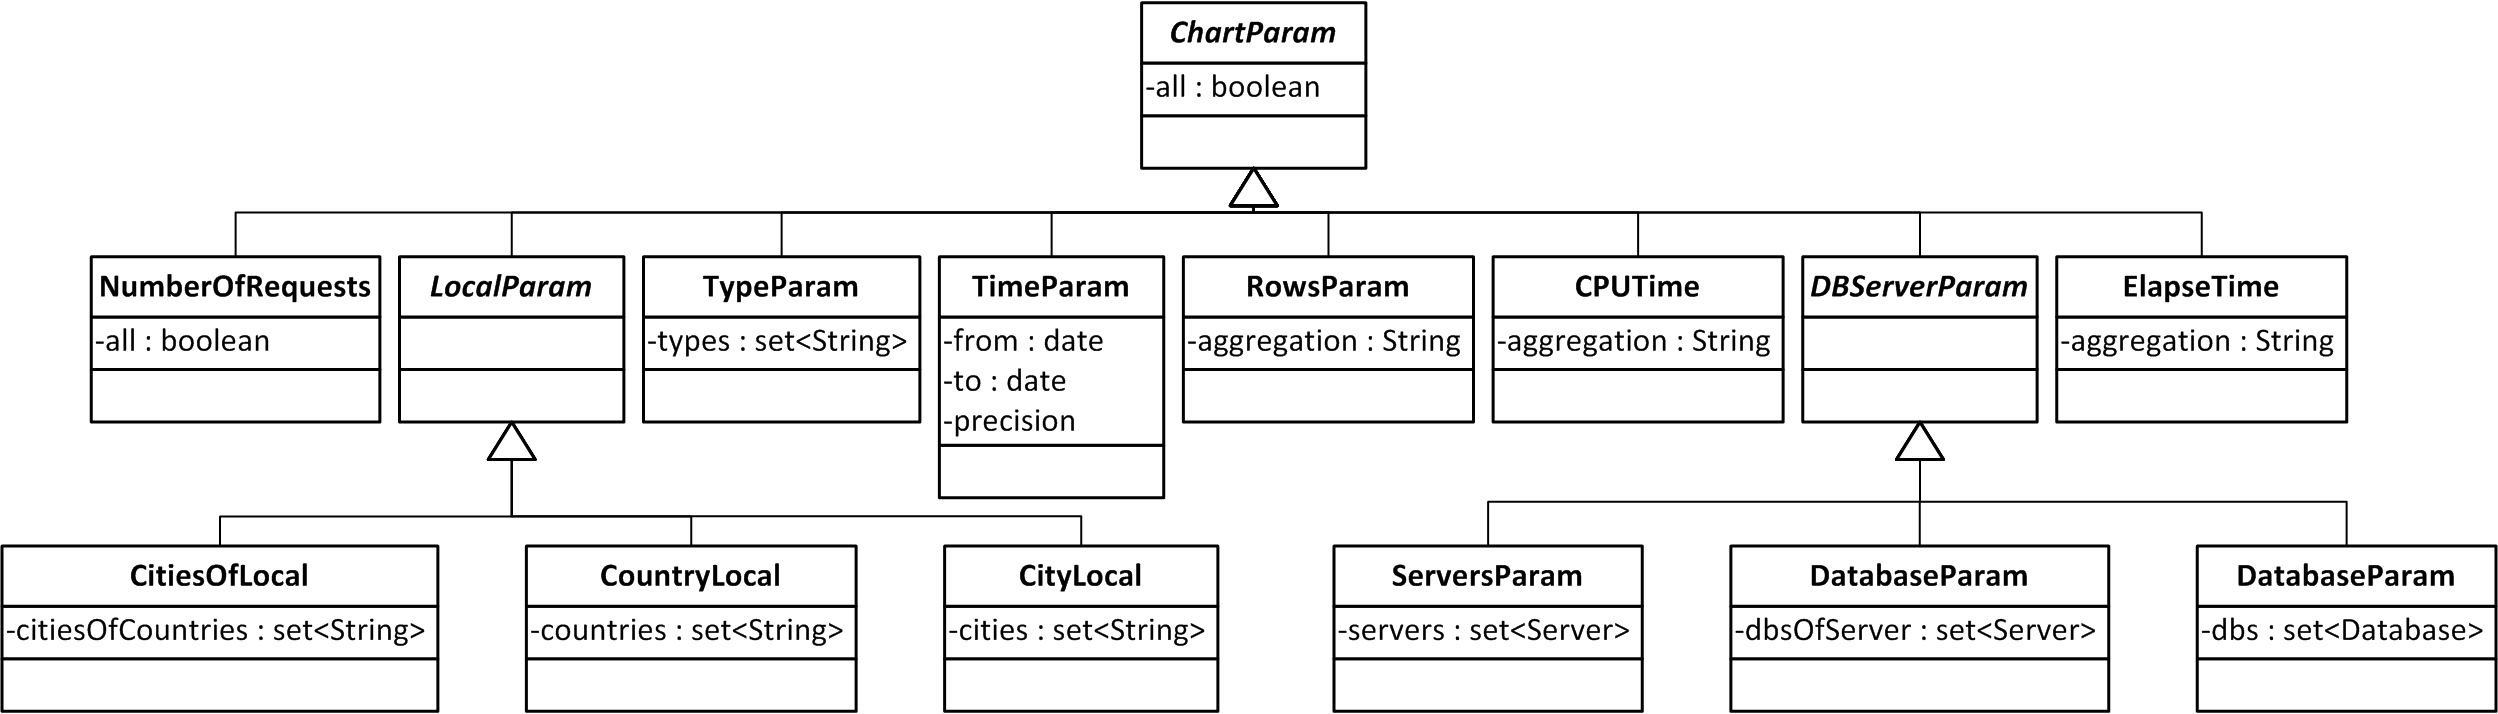
\includegraphics[width=1\linewidth]{Pictures/Parts/ChartPara.png}
\end{center}  

\subsubsection*{ChartParam}  
ChartParam represent on the one hand the type of a dimension or measure, like time or number of rows, and
on the other hand the interval or the aggregation. e.g. sum or maximum, requested or filtered. %not clear, for me anyways :D
With the boolean set true may be shown, that no filtering is required on this parameter, or, if implemented
an other way, they may be just left out in that case. 
This ChartParam stand just representative for possible chart parameter and may be implemented way more dynamically.



%=||======================================================================>
\newpage
\subsection{Parser}

\begin{center}
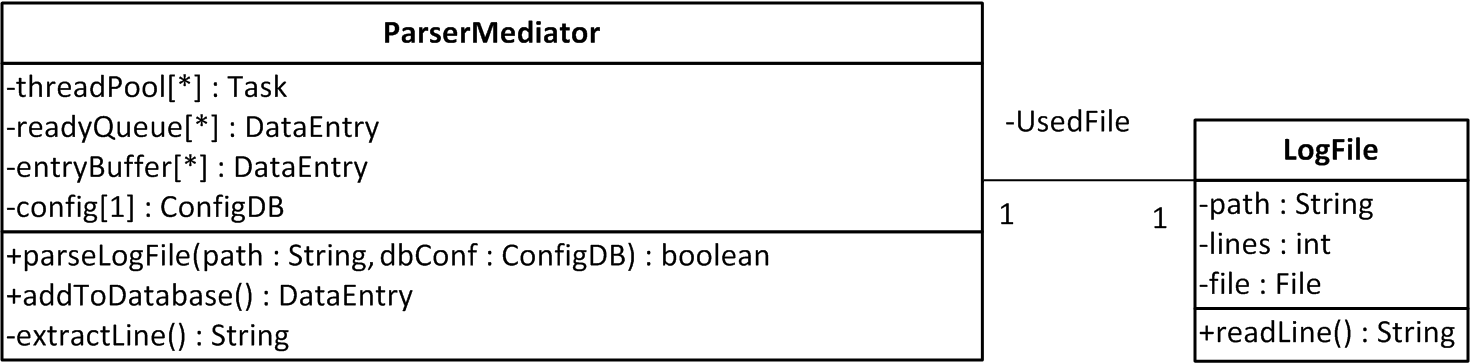
\includegraphics{Pictures/Parts/ParsMedi.png}
\end{center}  

\subsubsection*{ParserMediator}
ParserMediator is the 'main'-Class of the Parser. It creates and administrates a threadpool,
 which contains several tasks, 
%contains used twice very shortly (I was momentarily confused).Also, the sentence is huge. I see no immediate replacement
contains the entryBuffer for finished DataEntries, the stringBuffer for strings,
which were extracted from the log file and saves which log file and configuration file is used.

\subsubsection*{LogFile}
The gateway between parser and log file - it contains the path of the logfile and an integer 
which saves how many lines have been read from this file. It can read single lines from the
logfile and return them to the Parser.

\begin{center}
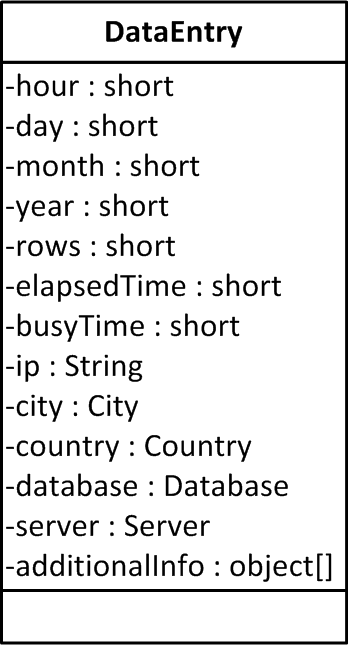
\includegraphics{Pictures/Parts/DataEntry.png}
\end{center}  

\subsubsection*{DataEntry}
The DataEntry stores the data which will be written into the warehouse. The given attributes stand representative
for possible for possible data. The implementation of them may be way more dynamically.

% It contains 
% -hour, day, month, year of the request,
% -rows which were read  from the logfile%from the logfile or rows accessed in the original db? %+1, it is not clear
% -the elapsed and busy time on the server
% -the ip from which the request came
% -the type of request
% -the database and server which handled the request. %I Thought I'd break this up and make a list
% It may contain additional information depending on the actual logfile, as specified in the configuration file. 
% %is this correct?

%\newline\newline doesnt work in empty lines
% \subsubsection*{Java Files}
% The Parser uses java.io.File and a ThreadPool from java.util.


\newpage
\begin{center}
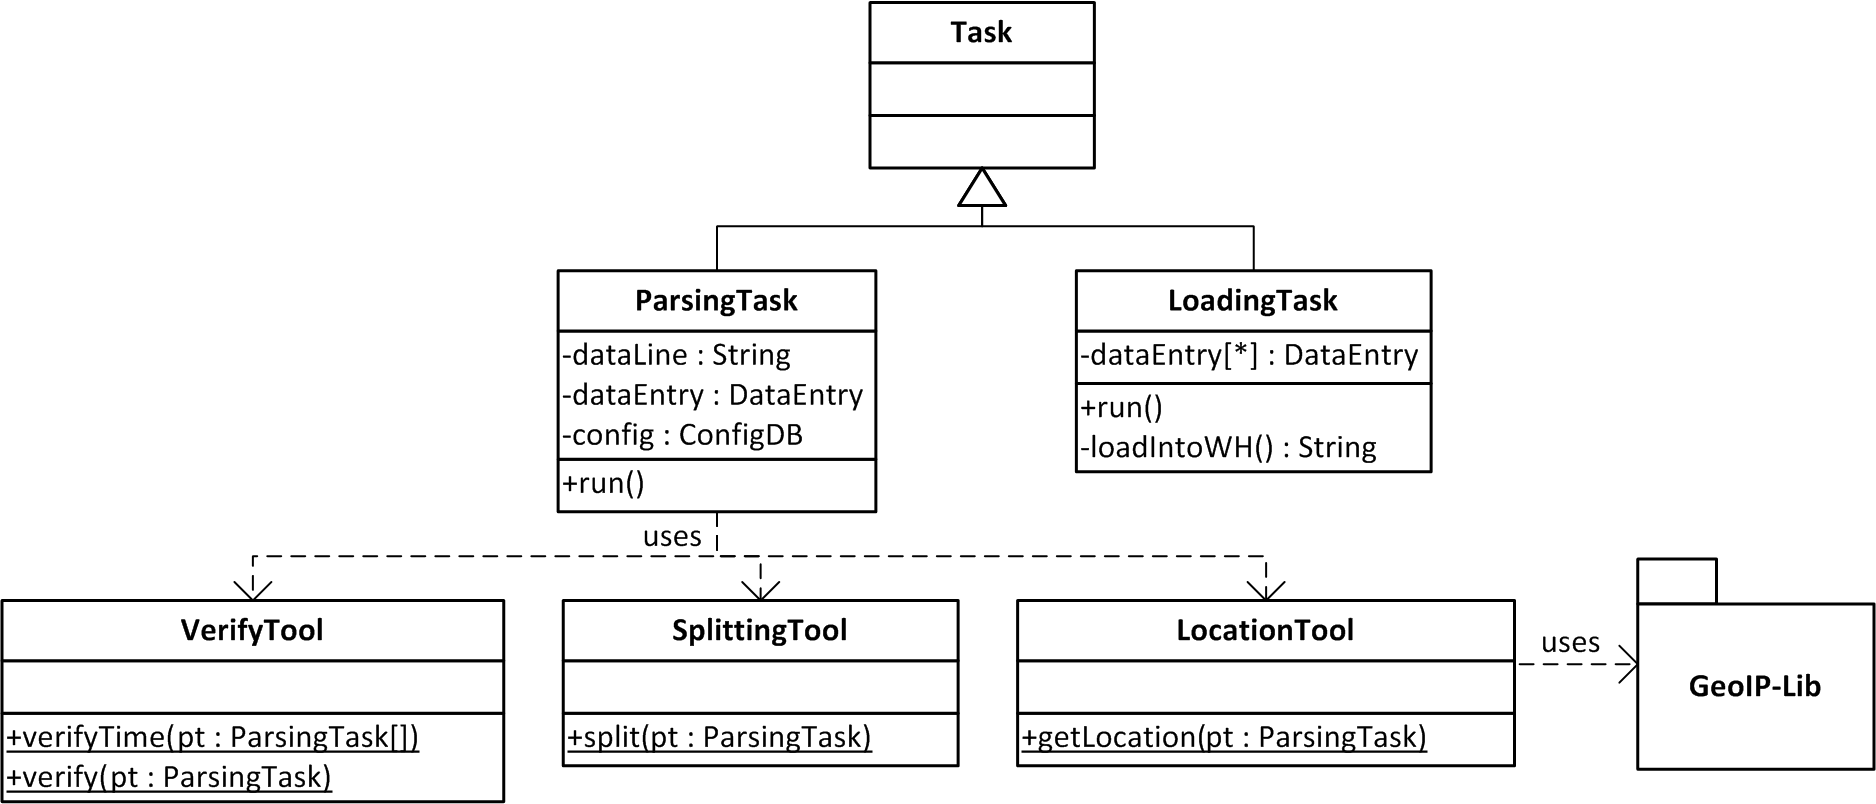
\includegraphics[width=1\linewidth]{Pictures/Parts/TaskTool.png}
\end{center}

\subsubsection*{ParsingTask}
ParsingTasks are tasks created by the ParserMediator. They receive a line from the log file and use  
SplittingTool, VerifyTool and LocationTool to create a DataEntry. 


\subsubsection*{SplittingTool}
The SplittingTool splits the dataLine from its parsingTask and enters the splitted raw parts into the DataEntry.

\subsubsection*{VerifyTool}
The VerifyTool checks the DataEntry for its correctness. % - if it has a mistake (e.g. Month = 13 or Elapsed Time = -1),
If mistakes are found this line will be deleted and a internal exception registrated. 

\subsubsection*{LocationTool}
The LocationTool uses GeoIP-Libraries (\ref{geo}) to determine the city and country of the request out of the ip.

\subsubsection*{LoadingTask}
A LoadingTask is another possible task for the thread pool.
It takes finished DataEntries from the buffer and sends them to the data access tier.




%=||======================================================================>
\newpage 
\subsection{Data access tier}

\begin{center}
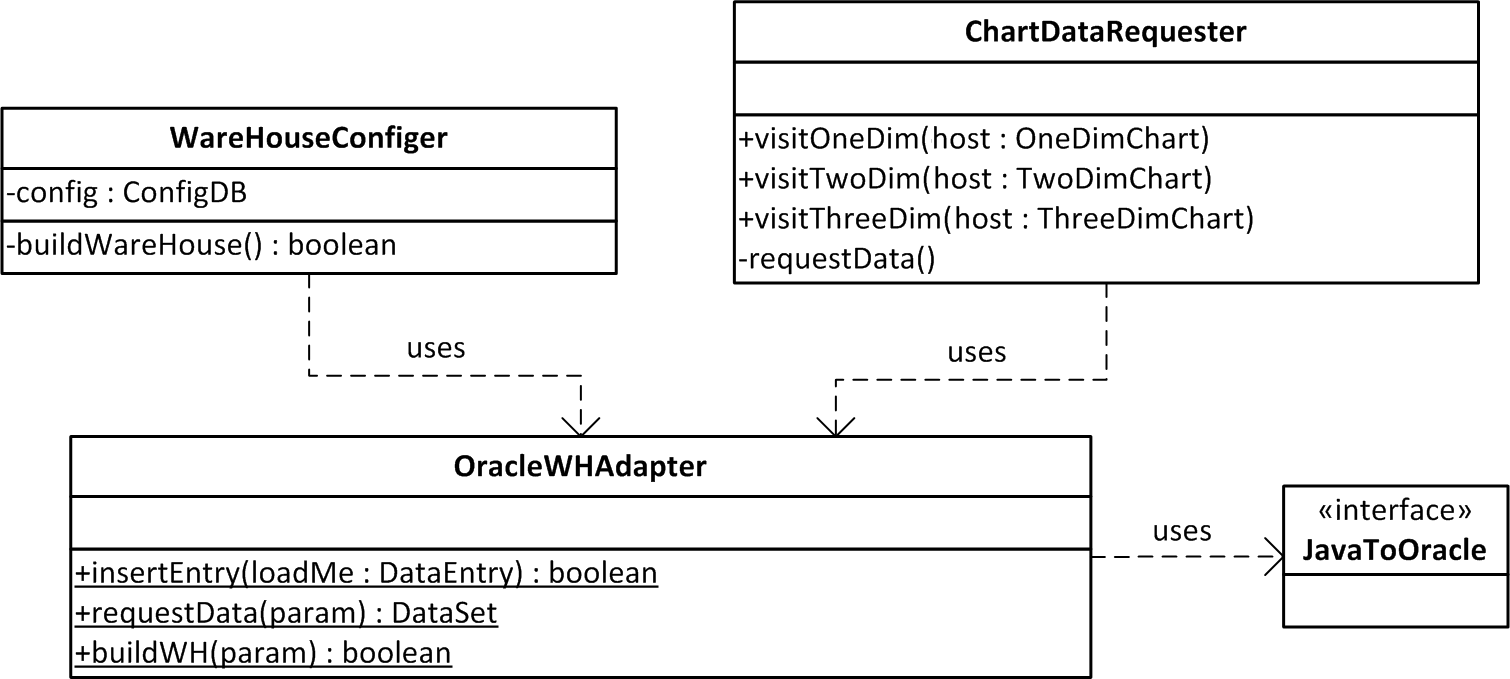
\includegraphics{Pictures/Parts/Data.png}
\end{center} 

\subsubsection*{ChartDataRequester}

The ChartDataRequester is the first of the three visitors of a ChartHost. Its task is to 
create the queries to gain the data needed for the charts. It takes the information about what he
has to request from the hosted ChartHost.


\subsubsection*{OracleWHAdapter}

Every query, whether loading, extracting or anything else, run against the Oracle server is made by this,
and only by this, class. So it represents the interface out of the application to the data.



\subsubsection*{JavaToOracle}

Any library used for the connection and communication with the Oracle server, 
where the Warehouse is stored. It is only used by the OracleWHAdapter.

 

\subsubsection*{WareHouseConfiger}

This class will only be needed if a very optional function will be implemented. It's task is to create
a warehouse for one certain new database just with the information of its configuration file information.

